\section{Directory Structure}
\label{sc_structure}

\Dumux has the following folder structure, which is similar to other \Dune modules.
\begin{itemize}
\item \texttt{bin}: contains binaries, e.g. used for the automatic testing
\item \texttt{cmake}: the configuration options for building \Dumux
\item \texttt{doc}: contains the Doxygen documentation (\texttt{doc/doxygen/html/index.html}),
                    this handbook, and various logos
\item \texttt{dumux}: the main folder, containing the source files, see \ref{fig:dumux-structure}
      for a visualized structure. For more information on the models have a look at the
      Doxygen documentation.
  \begin{itemize}
  \item \texttt{common}: general methods shared by all models, 
         like the \texttt{start.hh} or the time manager

  \item \texttt{decoupled}: contains sequential models (pressure equation as part of
         the fractional flow formulation). The general decoupled formulation can be found in
         the subdirectory \texttt{common}. In each model folder, there are subdirectories
         for the implicit pressure equation sorted by the employed discretization method,
         and for the explicit transport equation.

  \item \texttt{freeflow}: single-phase free-flow models. All models are discretized
         fully implicitly using the box-method.

  \item \texttt{geomechanics}: models for solving rock mechanics and flow.

  \item \texttt{implicit}: contains all fully implicit models. General methods shared
         by all models are contained in \texttt{common}, together with specilized methods
         for the two discretization types \texttt{box} and \texttt{cellcentered}. The
         \texttt{adaptive} folder contains methods for grid adaption. Each of the other
         subdirectories contain a derived specific numerical model.

  \item \texttt{io}: additional in-/output possibilities like restart files,
        gnuplot-interface and a VTKWriter.

  \item \texttt{linear}: contains linear solver backends.

  \item \texttt{material}: all material parameters and constitutive equations.
        Properties of a pure chemical (pseudo)substance (e.g. water, air) are located
        in \texttt{components}. The fluidsystems collect information from the \texttt{components} and
        \texttt{binarycoefficients} (like Henry coefficients), and combines them with fluid phase characteristics
        (e.g. viscosity, density).
        The folder \texttt{spatialparams} contains all spatially dependend variables, like permeability and porosity.
        The class in \texttt{implicitspatialparameters.hh} provides spatial averaging routines.
        Constitutive relations are found in \texttt{fluidmatrixinteractions},.

  \item \texttt{multidomain}: coupling handling and coupling conditions for connecting
        different model types in different subdomains.

  \item \texttt{nonlinear}: Newton's method.

  \item \texttt{parallel}: helper files for parallel simulations
\end{itemize}

\item \texttt{test}: tests for each numerical model and some functionality.
      The structure is equivalent to the dumux folder, the \texttt{references} folder
      contains solutions for the automatic testing. Each test program consist of source
      \texttt{*.cc}, the problem definition \texttt{*problem.hh}, the definition of the spatially dependent
      parameters \texttt{*spatialparameters.hh} and an input file \texttt{*problem.hh}.
      For more detailed descriptions of the tests, please have a look at the Doxygen documentation.

\item \texttt{tutorial}: contains the tutorials described in Chapter \ref{chp:tutorial}.
\end{itemize}

% \begin{figure}
\begin{sidewaysfigure}
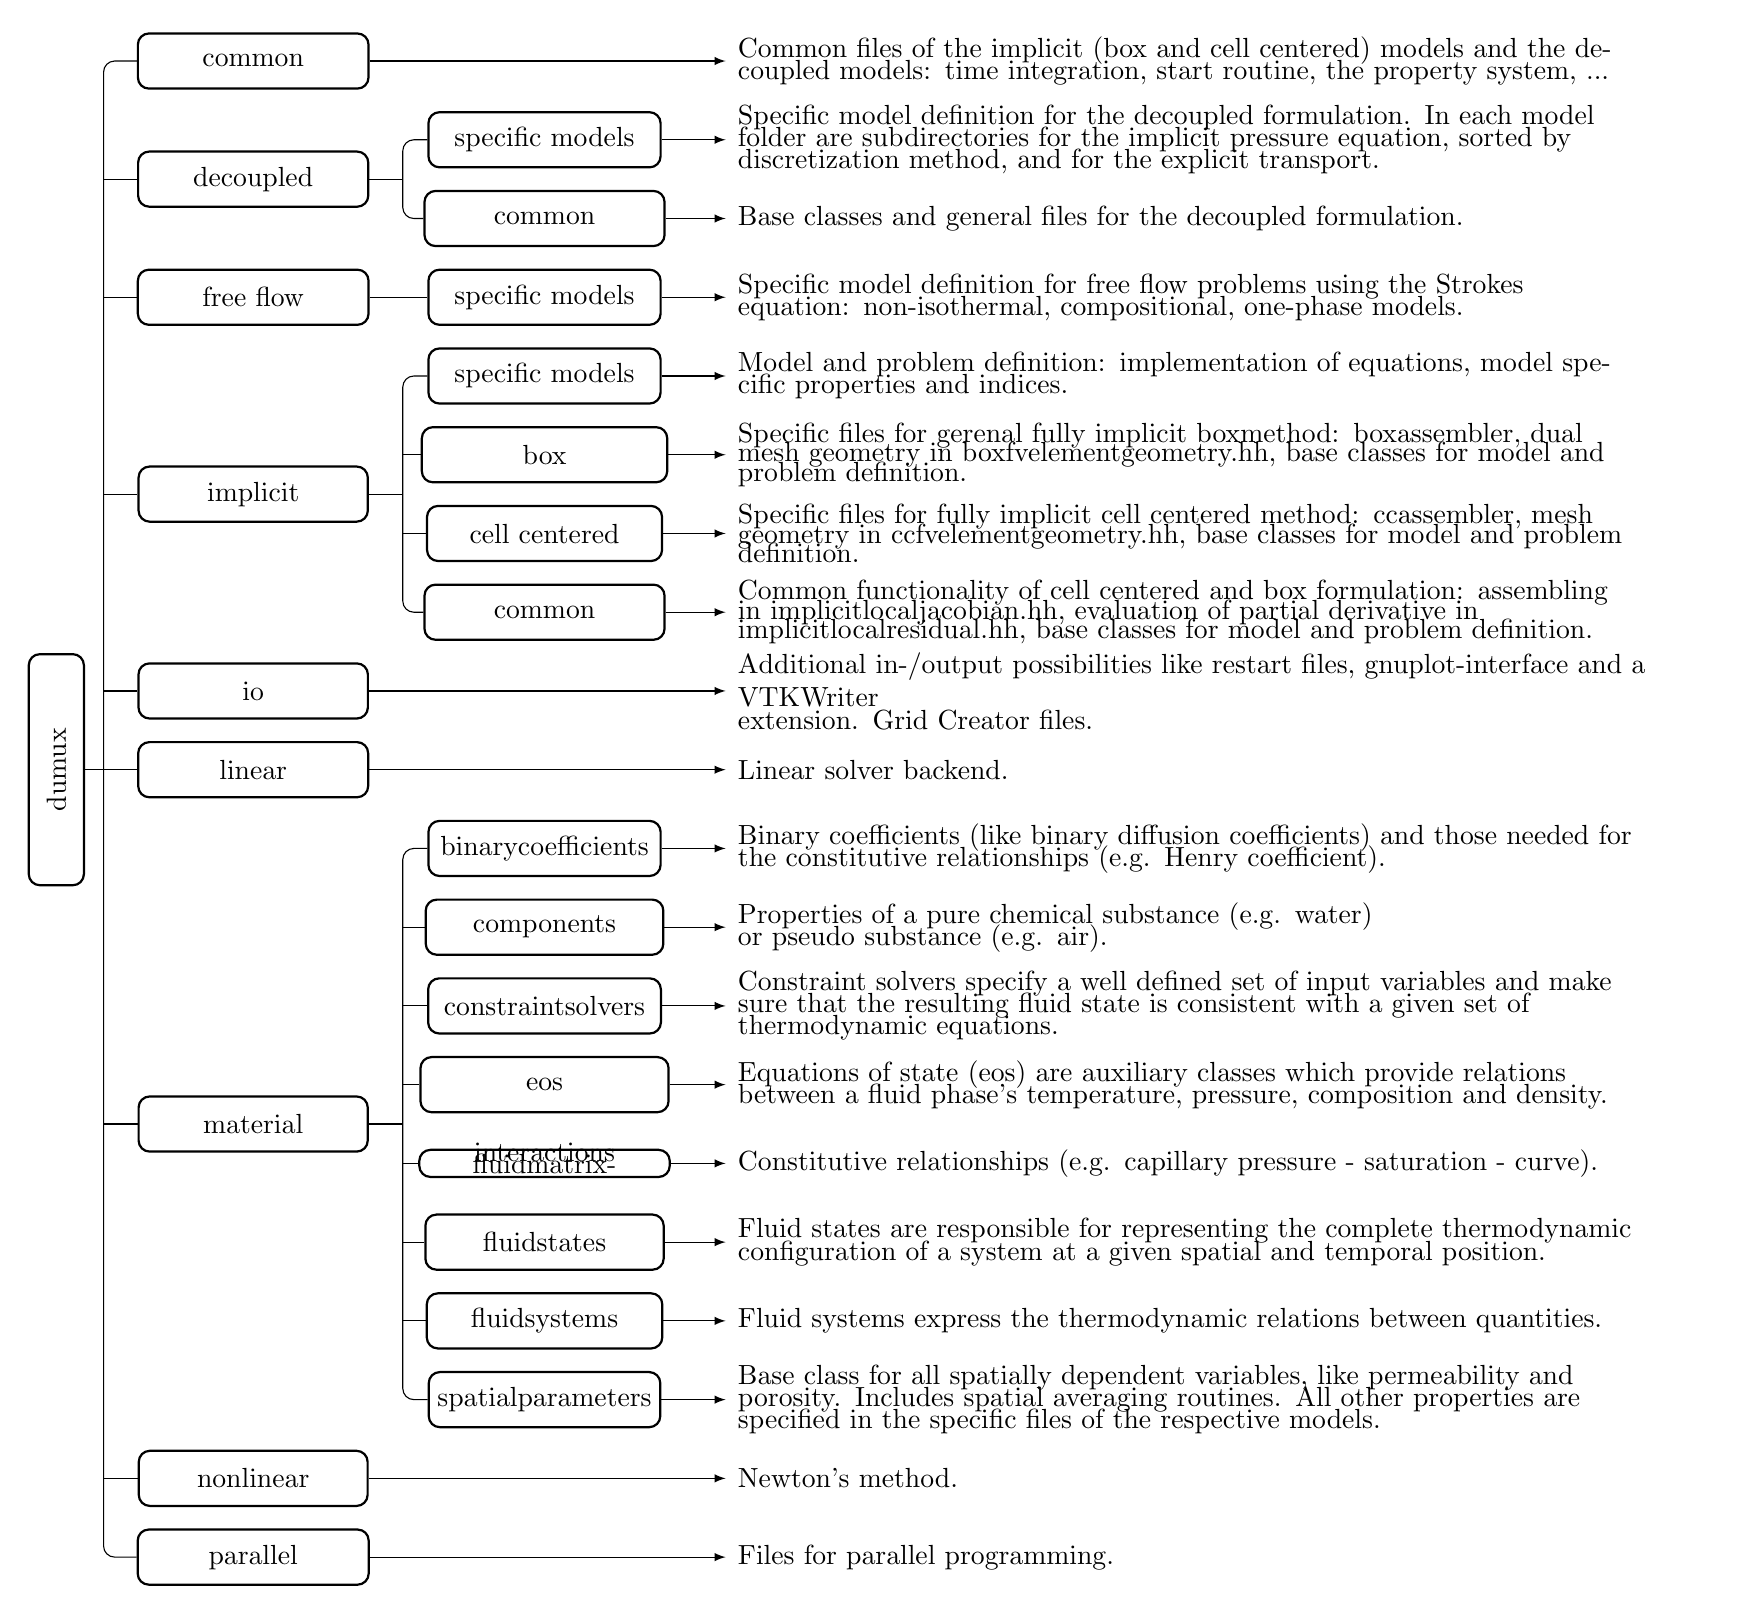
\begin{tikzpicture}[>=latex,inner xsep=0.15cm,rounded corners]
\node [minimum height=0.7cm,draw,inner xsep=0.94cm,rotate=90,thick] (d) at(-2,0) {dumux};
\node [minimum height=0.7cm,draw,inner xsep=1.03cm,thick] (lin) at(0.5,0) {linear};
\node [minimum height=0.7cm,draw,inner xsep=1.32cm,thick] (io) at(0.5,1) {io};

\node [minimum height=0.7cm,draw,inner xsep=0.87cm,thick] (imp) at(0.5,3.5) {implicit};
 \node [minimum height=0.7cm,draw,inner xsep=0.88cm,thick] (c1) at(4.2,2) {common};
 \node [minimum height=0.7cm,draw,inner xsep=0.54cm,thick] (cell) at(4.2,3) {cell centered};
 \node [minimum height=0.7cm,draw,inner xsep=1.28cm,thick] (box) at(4.2,4) {box};
 \node [minimum height=0.7cm,draw,inner xsep=0.33cm,thick] (spec1) at(4.2,5) {specific models};

\node [minimum height=0.7cm,draw,inner xsep=0.82cm,thick] (free) at(0.5,6) {free flow};
  \node [minimum height=0.7cm,draw,inner xsep=0.33cm,thick] (spec2) at(4.2,6) {specific models};

\node [minimum height=0.7cm,draw,inner xsep=0.7cm,thick] (dec) at(0.5,7.5) {decoupled};
 \node [minimum height=0.7cm,draw,inner xsep=0.88cm,thick] (c2) at(4.2,7) {common};
 \node [minimum height=0.7cm,draw,inner xsep=0.33cm,thick] (spec3) at(4.2,8) {specific models};

\node [minimum height=0.7cm,draw,inner xsep=0.82cm,thick] (c3) at(0.5,9) {common};

\node [minimum height=0.7cm,draw,inner xsep=0.82cm,thick] (m) at(0.5,-4.5) {material};
 \node [minimum height=0.7cm,draw,thick] (bin) at(4.2,-1) {binarycoefficients};
 \node [minimum height=0.7cm,draw,inner xsep=0.6cm,thick] (comp) at(4.2,-2) {components};
 \node [minimum height=0.7cm,draw,inner xsep=0.2cm,thick] (con) at(4.2,-3) {constraintsolvers};
 \node [minimum height=0.7cm,draw,inner xsep=1.34cm,thick] (eos) at(4.2,-4) {eos};
 \node [inner ysep=0.05cm,draw,text width=2cm,align=center,inner xsep=0.59cm,thick] (fi) at(4.2,-5) {fluidmatrix-\\[-16pt]interactions};
 \node [minimum height=0.7cm,draw,inner xsep=0.73cm,thick] (fstate) at(4.2,-6) {fluidstates};
 \node [minimum height=0.7cm,draw,inner xsep=0.56cm,thick] (fsys) at(4.2,-7) {fluidsystems};
 \node [minimum height=0.7cm,draw,inner xsep=0.11cm,thick] (s) at(4.2,-8) {spatialparameters};

\node [minimum height=0.7cm,draw,inner xsep=0.74cm,thick] (non) at(0.5,-9) {nonlinear};
\node [minimum height=0.7cm,draw,inner xsep=0.9cm,thick] (para) at(0.5,-10) {parallel};

\draw (d)--(lin);
\draw (-1.4,0)--(-1.4,9)--(c3);
\draw (-1.4,0)--(-1.4,-10)--(para);
\draw (-1.4,7.5)--(dec);
\draw (-1.4,6)--(free);
\draw (-1.4,3.5)--(imp);
\draw (-1.4,1)--(io);
\draw (-1.4,-4.5)--(m);
\draw (-1.4,-9)--(non);

\draw (dec)--(2.4,7.5);
\draw (spec3)--(2.4,8)--(2.4,7)--(c2);
\draw (free)--(spec2);
\draw (imp)--(2.4,3.5);
\draw (spec1)--(2.4,5)--(2.4,2)--(c1);
\draw (box)--(2.4,4);
\draw (cell)--(2.4,3);
\draw (m)--(2.4,-4.5);
\draw (bin)--(2.4,-1)--(2.4,-8)--(s);
\draw (comp)--(2.4,-2);
\draw (con)--(2.4,-3);
\draw (eos)--(2.4,-4);
\draw (fi)--(2.4,-5);
\draw (fstate)--(2.4,-6);
\draw (fsys)--(2.4,-7);

\draw [->](c3)--(6.5,9) node [right,text width=12.5cm,align=left]
  {Common files of the implicit (box and cell centered) models and the de-\\[-4pt]
   coupled models: time integration, start routine, the  property system, ...};
\draw [->](spec3)--(6.5,8) node [right,text width=12.5cm,align=left]
  {Specific model definition for the decoupled formulation. In each model \\[-4pt]
   folder are subdirectories for the implicit pressure  equation, sorted by \\[-4pt]discretization method, and for the explicit transport.};
\draw [->](c2)--(6.5,7) node [right,text width=12.5cm,align=left]
  {Base classes and general files for the decoupled formulation.};
\draw [->](spec2)--(6.5,6) node [right,text width=12.5cm,align=left]
  {Specific model definition for free flow problems using the Strokes \\[-4pt]
   equation: non-isothermal, compositional, one-phase models.};
\draw [->](spec1)--(6.5,5) node [right,text width=12.5cm,align=left]
  {Model and problem definition: implementation of equations, model spe-\\[-4pt]
   cific properties and indices.};
\draw [->](box)--(6.5,4) node [right,text width=12.5cm,align=left]
  {Specific files for gerenal fully implicit boxmethod: boxassembler, dual \\[-5pt]
   mesh geometry in boxfvelementgeometry.hh, base classes for model and \\[-5pt]problem definition.};
\draw [->](cell)--(6.5,3) node [right,text width=12.5cm,align=left]
  {Specific files for fully implicit cell centered method: ccassembler, mesh \\[-5pt]
   geometry in ccfvelementgeometry.hh, base classes for model and problem \\[-5pt]definition.};
\draw [->](c1)--(6.5,2) node [right,text width=12.5cm,align=left]
  {Common functionality of cell centered and box formulation: assembling \\[-5pt]
   in implicitlocaljacobian.hh, evaluation of partial derivative in \\[-5pt]implicitlocalresidual.hh, base classes for model and problem definition.};
\draw [->](io)--(6.5,1) node [right,text width=12.5cm,align=left]
  {Additional in-/output possibilities like restart files, gnuplot-interface and a VTKWriter \\[-4pt]
   extension. Grid Creator files.};
\draw [->](lin)--(6.5,0) node [right,text width=12.5cm,align=left] {Linear solver backend.};
\draw [->](bin)--(6.5,-1) node [right,text width=12.5cm,align=left]
  {Binary coefficients (like binary diffusion coefficients) and those needed for \\[-4pt]
   the constitutive relationships (e.g. Henry coefficient).};
\draw [->](comp)--(6.5,-2) node [right,text width=12.5cm,align=left]
  {Properties of a pure chemical substance (e.g. water) \\[-4pt]or pseudo substance (e.g. air).};
\draw [->](con)--(6.5,-3) node [right,text width=12.5cm,align=left]
  {Constraint solvers specify a well defined set of input variables and make \\[-4pt]
   sure that the resulting fluid state is consistent with a given set of \\[-4pt]thermodynamic equations.};
\draw [->](eos)--(6.5,-4) node [right,text width=12.5cm,align=left]
  {Equations of state (eos) are auxiliary classes which provide relations \\[-4pt]
   between a fluid phase's temperature, pressure, composition and density.};
\draw [->](fi)--(6.5,-5) node [right,text width=12.5cm,align=left]
  {Constitutive relationships (e.g. capillary pressure - saturation - curve).};
\draw [->](fstate)--(6.5,-6) node [right,text width=12.5cm,align=left]
  {Fluid states are responsible for representing the complete thermodynamic \\[-4pt]
   configuration of a system at a given spatial and temporal position.};
\draw [->](fsys)--(6.5,-7) node [right,text width=12.5cm,align=left]
  {Fluid systems express the thermodynamic relations between quantities.};
\draw [->](s)--(6.5,-8) node [right,text width=12.5cm,align=left]
  {Base class for all spatially dependent variables, like permeability and \\[-4pt]
   porosity. Includes spatial averaging routines. All other properties are \\[-4pt]
   specified in the specific files of the respective models.};
\draw [->](non)--(6.5,-9) node [right,text width=12.5cm,align=left]
  {Newton's method.};
\draw [->](para)--(6.5,-10) node [right,text width=12.5cm,align=left]
  {Files for parallel programming.};
\end{tikzpicture}
\caption{Structure of the directory \texttt{dumux} containing the \Dumux source files.
          \todo[inline]{Diese Skizze ist NICHT mehr aktuell. Hochkant passt sie wahrscheinlich besser auf die Seite.
                        Neue Tikz Templates sollten eingführt werden. Eventuell Grafik/Schrift verkleinern und einpassen.
                        Eventuell mit nur relative Platzierung der Boxen mit lower-of ... (Thomas)}}
\label{fig:dumux-structure}
\end{sidewaysfigure}
% \end{figure}
